%!TEX root = ./template-skripsi.tex
%-------------------------------------------------------------------------------
%                     BAB III
%               			PEMBAHASAN
%-------------------------------------------------------------------------------

\chapter{METODOLOGI PENELITIAN}

\section{Tahapan Penelitian}

Gambar \textit{flowchart} berikut mengilustrasikan proses pelatihan 
 dari dataset dan juga proses penggunaan yang sesungguhnya.

\begin{figure}[H]
  \centering{}
	\includegraphics[width=0.6\textwidth]{gambar/flowchart\_1\_1}
  \caption{Diagram alir untuk algoritma pelatihan klasifikasi objek}
\end{figure}

\begin{figure}[H]
  \centering{}
	\includegraphics[width=0.6\textwidth]{gambar/flowchart\_2}
  \caption{Diagram alir untuk algoritma pendeteksian objek}
\end{figure}

%(Jelasin disini secara ringkas, biar gak terlalu ambigu)

\section{Desain Sistem}

Dalam proses pembuatan \emph{classifier} perlu dilewati tahapan \textit{training}. 
Tujuan \textit{training} adalah untuk menciptakan suatu \emph{strong classifier} 
yang nantinya dapat digunakan untuk melakukan klasifikasi yang sebenarnya.
Pertama, gambar yang akan menjadi \textit{set} latihan dianotasi sesuai kelasnya masing-masing, 
\textit{set} latihan ini juga berisikan gambar-gambar yang tidak memiliki kelas yang benar, atau 
\emph{false example}. Setelah itu gambar melalui proses \emph{pre-processing} dan disesuaikan 
untuk mengoptimalkan proses pelatihan. Setiap gambar latihan nantinya akan 
diubah menjadi \emph{integral image} untuk dapat diproses.

Pertama algoritma akan mengkonstruksi sebuah \emph{decision tree} untuk setiap 
\emph{weaklearn} dimana \emph{branch} untuk setiap kelas akan ditentukan. Lalu 
\emph{Adaboost} akan menentukan bobot dari setiap \emph{weaklearn} dalam menentukan hasil akhir 
klasifikasi gambar. Terakhir, \emph{Adaboost} akan membuat sebuah 
\emph{strong classifier} dengan membuat sebuah \emph{Attentional Cascade}

Dengan \emph{strong classifier}, klasifikasi objek yang sesungguhnya bisa dilakukan. 
Pertama gambar yang akan dideteksi akan melalui \emph{pre-processing}. 
Kemudian \emph{integral image} akan dihitung untuk 
menghasilkan \emph{sub-window} pada gambar. setiap sub-window akan dicek menggunakan 
\emph{strong classifier}. \emph{Sub-window} yang ditemukan memiliki objek yang 
dicari akan dibuatkan \emph{bounding box} pada kelilingnya. Setelah semua 
\emph{sub-window} diperiksa, semua \emph{bounding box} yang bertindihan akan 
digabungkan sebelum gambar hasil dikembalikan ke pengguna.

\section{Training \emph{Strong Classifier}}

Pada \textit{Training} ada tiga tahapan yang perlu dijalankan 
untuk menghasilkan sebuah \emph{Strong Classifier}, 
yaitu penginputan \textit{dataset} pelatihan yang sudah dianotasi, 
pembuatan \emph{decision tree} untuk setiap fitur, 
\emph{Boosting }dan pemilihan fitur oleh Adaboost untuk membuat \emph{attentional cascade}.

\subsection{\textit{Input Dataset} Pelatihan}

\begin{figure}[H]
  \centering{}
	\includegraphics[width=0.6\textwidth]{gambar/dataset\_2}
  \caption{Contoh gambar Abudefduf, Amphiprion, Chaetodon dan contoh gambar-gambar negatif}
\end{figure}

\textit{Dataset} yang akan dipakai diambil dari fishR (Dapat dilihat di https://github.com/mekas/fishR) yang 
berisikan gambar ikan genus Abudefduf, Amphiprion dan Chaetodon. Selain itu 
\textit{dataset} juga akan ditambahkan dari hasil penelitian lapangan 
secukupnya, dengan mempertimbangkan waktu komputasi pada tahap 
pelatihan.
Untuk contoh pelatihan kelas-kelas ikan adalah gambar berukuran 72x41 piksel, 
dengan warna grayscale. Selain itu juga akan dipilih contoh 
pelatihan negatif atau kumpulan gambar yang tidak terdapat kelas 
ikan dari http://www.vision.caltech.edu/datasets/ dengan jumlah yang sama, resolusi sama dan perlakuan 
yang sama. Anotasi dilakukan dengan rumus $(x_1, y_1),...,(x_n, y_n)$ dimana 
$y_i \in Y = {1,...,k}$, $k$ disini adalah kelas-kelas yang ada dimana $y_i = 0$ 
direservasi untuk kelas negatif dan angka-angka setelahnya untuk kelas-kelas lainnya.
\textit{Dataset} ini lalu 
akan dibagi menjadi tiga yaitu \textit{training dataset}, 
\textit{validation dataset}, dan \emph{test dataset} dengan jumlah yang sama.
Nilai bobot pada tiap \textit{dataset} akan di inisialisasi dengan rumus:
\begin{equation}
  w^1_i = D(i) \text{ for } i=1,...,N
\end{equation}
dimana $w$ adalah bobot, $D$ Distribusi dan $N$ jumlah contoh pelatihan.

\subsection{Pembuatan \textit{Integral Image}}

Untuk pembuatan \emph{Integral Image}, pertama perlu dicari nilai piksel
baris pertama dan kolom pertama dari gambar. Nilai pada matriks \emph{Integral Image} 
adalah median dari nilai RGB pada piksel tersebut, namun dikarenakan warna 
gambar sudah dirubah menjadi \emph{greyscale} maka nilai pada setiap piksel 
hanya akan berupa bilangan bulat dikisaran 0 sampai 255. Nilai pada kolom 
pertama hanyalah penjumlahan nilai piksel dari piksel $(0, 0)$ sampai ke piksel 
$(0, j)$, sementara nilai pada baris pertama juga hanya penjumlahan nilai 
piksel dari $(0, 0)$ ke  $(i, 0)$. Nilai-nilai piksel lainnya lalu dapat 
dihitung menggunakan rumus: 
\begin{equation}
  \begin{split}
    \text{integral image } (i,j) = {} & \text{integral image } (i-1,j) + \text{integral image } (i,j-1) - \\
    & \text{integral image } (i-1,j-1) + \text{nilai dari piksel } (i,j)
  \end{split}
\end{equation}
Atau jumlah semua nilai piksel dari $(0, 0)$ sampai ke $(i, j)$.
Pembuatan \emph{integral image} nantinya akan digunakan oleh fitur sebagai \textit{input}.

\begin{figure}[H]
  \centering{}
	\includegraphics[width=0.6\textwidth]{gambar/integral\_image\_3}
  \caption{Gambaran \emph{integral image} dari gambar sebuah bidak catur.}
\end{figure}

\subsection{Pembuatan \textit{like Features}}

Fitur-fitur yang akan digunakan dalam klasifikasi dibuat 
berdasarkan \emph{Haar-like Features} dan berisikan informasi 
lokasinya pada \emph{sub-window} dan titik-titik \emph{integral image}. 
Misalnya sebuah fitur dua persegi dengan persegi putih di 
sebelah kiri, fitur tersebut memerlukan 
nilai \emph{integral image} dari pojok kiri atas persegi putih, 
pojok kiri bawah persegi putih,  
pojok kanan atas persegi putih, 
pojok kanan bawah persegi putih, 
, pojok kanan atas persegi hitam, 
dan pojok kanan bawah persegi hitam. 
\begin{figure}[H]
  \centering{}
	\includegraphics[width=0.6\textwidth]{gambar/integral\_image\_4}
  \caption{Nilai yang diperlukan oleh fitur dua persegi, direpresentasi sebagai A, B, C, dan D}
\end{figure} 
Keenam nilai tersebut dapat digunakan untuk mencari nilai 
fitur dengan rumus:

\begin{equation}
  \begin{split}
    &\text{integral image E} - \text{integral image B} - \text{integral image D} + \text{integral image A} \\
    & - \text{integral image F} - \text{integral image C} - \text{integral image E} + \text{integral image B} \\    
  \end{split}
\end{equation}

Pada tahap ini fitur yang dipilih akan dibuat untuk semua 
posibilitas lokasi yang ada dan ukuran yang ada. Hal ini dilakukan dengan 
membuat fitur dimulai dari kiri atas gambar dengan ukuran 20 x 20 piksel untuk fitur 
dua persegi, dan 20 x 30 piksel untuk fitur tiga persegi, sampai pojok kanan bawah. 
Hal ini juga dilakukan sampai ukuran fitur lebih besar 
dari \emph{sub-window} yang digunakan dan tidak bisa muat lagi didalannya. 
Ukuran paling kecil dari fitur akan disesuaikan pada saat penelitian 
bila ternyata fitur terlalu banyak dan memperlambat proses pelatihan. 
Selain fitur dua persegi, akan juga dibuat beberapa fitur lainnya seperti, fitur 
tiga persegi dan empat persegi diagonal.

\subsection{Pembuatan \textit{Decision Tree}}

Setiap \emph{weaklearner} adalah sebuah \emph{decision tree} yang mengambil nilai 
dengan fitur sebagai variabel klasifikasi.
fitur dapat digunakan untuk mengembalikan 
sebuah nilai perbandingan intensitas cahaya dari suatu area pada gambar dan 
mendeteksi keberadaan suatu \emph{fitur} seperti 
perbedaan warna, garis, maupun perbedaan kontras pada gambar. Hal ini 
dilakukan dengan membaca nilai dari \emph{integral image}, yang merupakan 
representasi gambar, dan menghitung nilai dari fitur tersebut.
%(Jelasin step by step pembuatan decision tree pake algoritma).

Nilai yang didapat dari membaca \emph{integral image} menggunakan fitur lalu 
akan menjadi variabel pengetesan menggunakan \emph{decision tree}. Pada tahap ini 
semua \emph{decision tree} akan dilatih untuk mencari nilai \textit{branch} yang 
paling optimal, hal ini dilakukan dengan menggunakan gambar-gambar pada \textit{dataset} 
pelatihan sebagai input. \emph{Decision tree} yang dihasilkan pada tahap ini, 
bersamaan dengan fitur yang berhubungan dengannya, adalah \emph{weaklearner} 
yang akan digunakan untuk pembuatan \emph{Strong Classifier} pada tahap 
\emph{Boosting}.


\subsection{\emph{Boosting}}

Algoritma \emph{Adaboost} akan mem-\emph{boosting} \emph{weaklearner} untuk 
menciptakan sebuah \emph{strong classifier}. \emph{Boosting} dilakukan dari 
\emph{weaklearner} yang memiliki tingkat akurasi paling tinggi, dan dengan 
menggunakan \emph{dataset} latihan.

\emph{Adaboost} akan menjalankan \emph{weaklearner} terbaik untuk 
mengklasifikasi seluruh contoh \emph{dataset} latihan dan mencatat contoh yang 
gagal diklasifikasi oleh \emph{weaklearner} tersebut. 
Nilai dari \emph{weaklearner} 
tersebut dihitung dengan:
\begin{equation}
  sum(N)(i=1) w^t_i.1(h(x_i)\ne y_i)
\end{equation} 
dimana $N$ adalah jumlah total contoh latihan, $D_t$ adalah distribusi bobot pada 
iterasi $t$, $w^t_i$ adalah nilai bobot contoh ke-$i$ pada iterasi $t$, 
$y_i$ adalah label yang benar untuk contoh latihan ke-$i$, dan $h(x_i)$ 
adalah hasil dari \emph{weaklearn}. 
Hasilnya juga akan dicatat untuk urutan \emph{Boosting} ronde berikutnya dan 
juga sebagai nilai voting pada klasifikasi yang sebenarnya. 
Nantinya bobot dari seluruh \emph{dataset} latihan akan dihitung ulang dengan menaikan bobot dari contoh 
yang gagal diklasifikasi oleh \emph{weaklearner} sebelumnya. Proses ini dilakukan 
untuk setiap \emph{weaklearner}. 
%(Masukin rumus re-distribusi bobot contoh disini)

Ketika sebuah ronde \emph{Boosting} sudah selesai dan seluruh \emph{weaklearner} sudah  diurutkan sesuai dengan 
nilai yang didapat dari ronde tersebut. \emph{Adaboost} akan melakukan validasi 
tingkat akurasi \emph{strong classifier} yang sudah dibuat menggunakan \emph{dataset} validasi. 
hal ini dilakukan dengan membandingkan tingkat presisi \emph{strong classifer} 
yang dihasilkan ronde ini dengan \emph{strong classifer} yang dihasilkan ronde 
sebelumnya. Bisa tingkat presisi ternyata semakin berkurang, maka \emph{Boosting} 
akan dihentikan dan \emph{strong classifier} 
%(ronde ini atau sebelumnya, cek lagi) 
menjadi \emph{Strong Classifier}.

\subsection{Pembuatan \emph{Attentional Cascade}}

\begin{figure}[H]
  \centering{}
	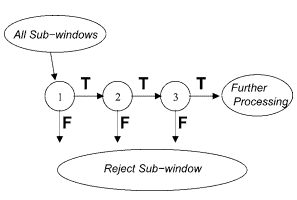
\includegraphics[width=0.6\textwidth]{gambar/cascade}
  \caption{\textit{Workflow} dari \emph{Attentional Cascade}}
\end{figure}

Sebelum pembuatan \emph{attentional cascade}, \emph{weaklearner} yang kurang 
diskriminatif akan dibuang dari \emph{Strong Classifier}. 
%Hal ini dilakukan dengan (cari, karena bagian ini 
%belum jelas dari kemarin). 
\emph{Attentional cascade} akan dibuat dari \emph{weaklearner} 
yang tersisa secara bertahap. 
Pertama, target \textit{false positive} pada setiap \emph{cascade} 
harus ditentukan oleh pengguna. \emph{Framework VIola-Jones} menggunakan target 
\textit{false positive} 50\% untuk \emph{cascade} pertama, dan 
\textit{false positive} 80\% untuk semua \emph{cascade} setelahnya.
Target \textit{false posiive} ini akan disesuaikan 
saat penelitian lapangan, bila target akurasi tidak berhasil dicapai 
dengan target \textit{false positive} sebelumnya.
Pada setiap fase \emph{cascade}, \emph{weaklearner} akan 
ditambahkan satu-persatu. Setiap sebuah \emph{weaklearner} ditambahkan, tes akan dilakukan 
dengan \emph{dataset} tes. \emph{Weaklearner} akan terus ditambahkan hingga \emph{false positive rate} 
yang ditentukan untuk fase itu dicapai. Fase akan terus bertambah hingga 
akurasi sempurna dicapai, atau hingga \emph{weaklearner} sudah habis. 
%(Ini periu dijabarin lagi dengan rumus per-step). 


\section{Skenario Eksperimen dan Validasi}

Tahapan ini adalah penggunakaan \emph{classifier} yang sebenarnya dengan tujuan 
memvalidasi akurasi dari \emph{classifier} tersebut. 
Gambar ikan yang akan dipakai dalam proses validasi akan 
melalui beberapa langkah dalam tahap ini, 
yaitu: \textit{Pre-processing} dalam bentuk \emph{grayscaling}, Penghitungan 
\emph{Integral Image}, dan deteksi yang sesungguhnya menggunakan \emph{strong classsifier} 
yang telah dibuat dengan metode Sliding Window.

\subsection{\textit{Pre-processing} dan Penghitungan \emph{Integral Image}}

Untuk klasifikasi sebenarnya, gambar \emph{input} akan diproses terlebih dahulu. 
Gambar awalnya akan melakui proses \textit{pre-processing} dan dirubah kedalam warna 
\emph{grayscale} %(Jelasin perubahan greyscale ini kayak gimana) 
untuk mempermudah penghitungan dengan bantuan \emph{library OpenCV}. 
Setelah tu sebuah matriks sebesar resolusi gambar akan dibuat untuk 
penghitungan \emph{Integral Image} yang nantinya akan mempercepat proses 
penghitungan fitur. Pembuatan \emph{integral image} pada tahap ini sama persis 
dengan pembuatan pada tahap pelatihan.

\subsection{Klasifikasi}

Pada tahap ini, gambar yang sudah berubah dalam bentuk 
\emph{integral image} akan diklasifikasi menggunakan 
\emph{strong classifier}. \emph{Strong classifier} akan berjalan dari 
pojok kiri atas gambar, atau piksel pertama, mencoba untuk mengklasifikasi 
sebuah \emph{sub-window} berukuran 72x41 piksel. Bila posisi tersebut sudah 
selesai diklasifikasi, terlepas hasilnya, \emph{sub-window} akan 
bergerak ke kanan sebanyak satu piksel dan mengklasifikasi area baru tersebut. 
Hal ini akan terus berlanjut hingga \emph{sub-window} bisa dibuat lagi ke kanan. 
Bilama demikian \emph{sub-window} akan kembali ke ka kanan, namun kali ini 
diturunkan sebanyak satu piksel. Pergerakan \emph{sliding window} ini 
bertujuan agar seluruh bagian dari gambar dapat terklasifikasi.

\begin{figure}[H]
  \centering{}
	\includegraphics[width=0.6\textwidth]{gambar/sliding\_window\_1}
  \caption{Gambaran ukuran \emph{sub-window} 72x41 piksel pada gambar 300x220}
\end{figure}

Jika \emph{sub-window} dengan ukuran 72x42 piksel sudah mengklasifikasi 
seluruh bagian gambar hingga pojok kanan bawah, maka \emph{sub-window} 
akan diperbesar dengan faktor 1.25 dan proses dimulai lagi dari pojok kiri atas. 
Selain itu ukuran dan lokasi dari \emph{feature} akan disesuaikan untuk mangakomodasi 
\emph{sub-window} yang sudah diperbesar. Hal ini dilakukan untuk mengklasifikasi 
objek yang memiliki ukuran berbeda didalam gambar.

\subsection{Anotasi}

\begin{figure}[H]
  \centering{}
	\includegraphics[width=0.6\textwidth]{gambar/sliding\_window\_2}
  \caption{Gambaran \textit{sub-window} yang berhasil mengklasifikasi ikan didalam gambar}
\end{figure}

Setelah semua \textit{sub-window} sudah diklasifikasi dengan menggunakan 
\emph{strong classifier}. Algoritma akan menggambarkan di lokasi \textit{sub-window} 
yang positif terklasifikasi (Memiliki salah satu kelas ikan yang telah dilatih ke \emph{strong classifier}), 
\emph{bounding box} untuk menganotasi kelasnya. Pengguna lalu dapat menentukan 
dari hasil anotasi bilamana target akurasi sudah tercapai.


